\documentclass[11pt, letterpaper]{article}

% ==========================================
% PACKAGES
% ==========================================
\usepackage{amsmath}
\usepackage{amssymb}
\usepackage{amsthm}
\usepackage{geometry}
\usepackage{tikz}
\usetikzlibrary{arrows.meta, positioning, shapes, automata, calc}
\usepackage{mathrsfs}
\usepackage{mathtools}
\usepackage{enumitem}
\usepackage{hyperref}
\usepackage{xcolor}
\usepackage{titlesec}

% ==========================================
% FORMATTING & GEOMETRY
% ==========================================
\geometry{margin=1in}
\setlength{\parindent}{0pt}
\setlength{\parskip}{0.5em}
\titleformat{\section}{\Large\bfseries\color{blue!60!black}}{\thesection}{1em}{}[{\titlerule[0.8pt]}]
\titleformat{\subsection}{\large\bfseries\color{black!80}}{\thesubsection}{1em}{}

% ==========================================
% THEOREM ENVIRONMENTS
% ==========================================
\newtheorem{theorem}{Theorem}[section]
\newtheorem{lemma}[theorem]{Lemma}
\newtheorem{proposition}[theorem]{Proposition}
\newtheorem{corollary}[theorem]{Corollary}
\theoremstyle{definition}
\newtheorem{definition}{Definition}[section]
\newtheorem{axiom}{Axiom}[section]
\newtheorem{example}{Example}[section]
\theoremstyle{remark}
\newtheorem{remark}{Remark}[section]

% ==========================================
% CUSTOM COMMANDS
% ==========================================
\newcommand{\E}{\mathbb{E}}
\newcommand{\Var}{\mathrm{Var}}
\newcommand{\Prob}{\mathbb{P}}
\newcommand{\R}{\mathbb{R}}
\newcommand{\N}{\mathbb{N}}
\newcommand{\F}{\mathcal{F}}
\newcommand{\ind}{\mathbf{1}}

% ==========================================
% DOCUMENT METADATA
% ==========================================
\title{\textbf{Homework 3: Discrete Probability Distributions and Waiting Times}}
\author{Tashfeen Omran}
\date{September 2026}

\begin{document}

\maketitle
\tableofcontents
\newpage

% ==========================================
% PART 1: INTRODUCTION
% ==========================================
\section{Part 1: Comprehensive Introduction, Context, and Prerequisites}

\subsection{Historical Context and Motivation}
The formalization of discrete probability distributions traces its roots to the 17th century, emerging from the correspondence between Blaise Pascal and Pierre de Fermat regarding gambling disputes, specifically the ``Problem of Points.'' Mathematicians sought to rigorously quantify the likelihood of sequences of events. Jacob Bernoulli's posthumous masterpiece, \textit{Ars Conjectandi} (1713), laid the rigorous foundation for what we now call Bernoulli trials and the Binomial distribution. The necessity to model not just a fixed number of trials, but the \textit{waiting time} until a certain number of successes occurs, naturally gave rise to the Geometric and Negative Binomial distributions. Today, these foundational concepts transcend gambling, serving as the bedrock for stochastic modeling in machine learning, algorithmic trading, and artificial intelligence.

\subsection{Core Concepts \& Axioms}
To treat discrete probability with the rigor of abstract mathematics, we must define our structures using measure theory. 

\begin{definition}[Probability Space]
A probability space is a measure space triplet $(\Omega, \F, \Prob)$, where:
\begin{itemize}
    \item $\Omega$ is the \textbf{sample space}, the set of all possible outcomes.
    \item $\F$ is a \textbf{$\sigma$-algebra} on $\Omega$, a collection of subsets of $\Omega$ containing $\Omega$ itself, closed under complementation and countable unions.
    \item $\Prob: \F \to [0, 1]$ is a \textbf{probability measure} satisfying Kolmogorov's Axioms: $\Prob(\Omega) = 1$, and for any countable sequence of pairwise disjoint sets $A_1, A_2, \dots \in \F$, $\Prob\left(\bigcup_{i=1}^\infty A_i\right) = \sum_{i=1}^\infty \Prob(A_i)$.
\end{itemize}
\end{definition}

\begin{definition}[Random Variable]
A discrete random variable $Y$ is an $\F$-measurable function $Y: \Omega \to S$, where $S \subset \R$ is countable. The probability mass function (PMF) is defined as $p(y) = \Prob(\{\omega \in \Omega : Y(\omega) = y\})$, often abbreviated as $\Prob(Y = y)$.
\end{definition}

In this chapter, we study experiments consisting of independent and identically distributed (i.i.d.) trials. Let $\Omega = \{S, F\}^n$ (for finite trials) or $\{S, F\}^\N$ (for infinite trials). We define a sequence of random variables $X_i: \Omega \to \{0, 1\}$ such that $X_i(\omega) = 1$ if the $i$-th trial is a success ($S$), and $0$ otherwise.

\subsection{Key Theorems, Lemmas, and Formulas}

\begin{theorem}[The Binomial Distribution]
Let $Y = \sum_{i=1}^n X_i$ be the number of successes in $n$ i.i.d. Bernoulli trials with success probability $p \in [0,1]$. Then $Y \sim \mathrm{Bin}(n, p)$, and its PMF is:
\[ p(y) = \binom{n}{y} p^y (1-p)^{n-y}, \quad y \in \{0, 1, \dots, n\} \]
Furthermore, $\E[Y] = np$ and $\Var(Y) = np(1-p)$.
\end{theorem}

\begin{theorem}[The Geometric Distribution]
Let $Y$ be the number of the trial on which the \textit{first} success occurs. Then $Y \sim \mathrm{Geom}(p)$, and its PMF is:
\[ p(y) = (1-p)^{y-1} p, \quad y \in \{1, 2, 3, \dots\} \]
Furthermore, $\E[Y] = \frac{1}{p}$ and $\Var(Y) = \frac{1-p}{p^2}$.
\end{theorem}

\begin{theorem}[The Negative Binomial Distribution]
Let $Y$ be the number of the trial on which the $r$-th success occurs. Then $Y \sim \mathrm{NB}(r, p)$, and its PMF is:
\[ p(y) = \binom{y-1}{r-1} p^r (1-p)^{y-r}, \quad y \in \{r, r+1, r+2, \dots\} \]
Furthermore, $\E[Y] = \frac{r}{p}$ and $\Var(Y) = \frac{r(1-p)}{p^2}$.
\end{theorem}

\subsection{Prerequisites}
Mastery of this topic requires:
1. \textbf{Set Theory:} Understanding partitions, intersections, and Cartesian products.
2. \textbf{Combinatorics:} Facility with binomial coefficients $\binom{n}{k} = \frac{n!}{k!(n-k)!}$.
3. \textbf{Real Analysis (Series):} Convergence of geometric series $\sum_{k=0}^\infty x^k = \frac{1}{1-x}$ for $|x| < 1$, and the ability to differentiate series term-by-term within their radius of convergence.

\newpage

% ==========================================
% PART 2: HOMEWORK SOLUTIONS
% ==========================================
\section{Part 2: Detailed Homework Solutions (Rigorous Proofs \& Computations)}

\textit{Note: Per the strategic selection protocol for advanced mathematical texts, we select a representative subset of problems that cover every distinct problem archetype (computation, algebraic manipulation, recursive proofs, and memoryless properties) to ensure complete conceptual mastery without redundant arithmetic repetition.}

\subsection{Problem 3.54: Symmetry of the Binomial Distribution}
\textbf{Problem Statement:} Suppose that $Y$ is a binomial random variable based on $n$ trials with success probability $p$ and consider $Y^* = n - Y$.
(a) Argue that for $y^* = 0, 1, \dots, n$, $\Prob(Y^* = y^*) = \Prob(Y = n - y^*)$.
(b) Use the result from part (a) to show that $\Prob(Y^* = y^*) = \binom{n}{y^*} q^{y^*} p^{n-y^*}$.
(c) Why is this result ``obvious''?

\begin{proof}[Solution to 3.54]
\textbf{Part (a):} We proceed by a direct set-theoretic equivalence. Let the underlying probability space be $(\Omega, \F, \Prob)$. The random variables $Y$ and $Y^*$ are mappings from $\Omega \to \R$. 
We are interested in the event $\{\omega \in \Omega : Y^*(\omega) = y^*\}$. 
By definition, $Y^*(\omega) = n - Y(\omega)$. Substituting this into the event condition yields:
\[ \{\omega \in \Omega : n - Y(\omega) = y^*\} = \{\omega \in \Omega : Y(\omega) = n - y^*\} \]
Since the underlying sets in the $\sigma$-algebra are identical, their probability measures must be equal:
\[ \Prob(Y^* = y^*) = \Prob(Y = n - y^*) \]

\textbf{Part (b):} We use the definition of the Binomial PMF. Let $q = 1-p$.
\[ \Prob(Y = y) = \binom{n}{y} p^y q^{n-y} \]
Substitute $y = n - y^*$ into the PMF:
\[ \Prob(Y^* = y^*) = \Prob(Y = n - y^*) = \binom{n}{n - y^*} p^{n - y^*} q^{n - (n - y^*)} \]
Simplify the exponent of $q$: $n - (n - y^*) = y^*$. 
Recall the combinatorial identity for binomial coefficients: $\binom{n}{k} = \frac{n!}{k!(n-k)!} = \binom{n}{n-k}$. Thus, $\binom{n}{n-y^*} = \binom{n}{y^*}$.
Substituting these back yields:
\[ \Prob(Y^* = y^*) = \binom{n}{y^*} q^{y^*} p^{n-y^*} \]

\textbf{Part (c):} The random variable $Y$ counts the number of ``successes'' in $n$ trials. Therefore, $Y^* = n - Y$ counts the number of ``failures'' in the same $n$ trials. If we simply redefine a ``failure'' (which occurs with probability $q$) as our new ``success'', the experiment is still a sequence of $n$ i.i.d. Bernoulli trials. Hence, $Y^*$ must follow a Binomial distribution with $n$ trials and success probability $q$.
\end{proof}

\subsection{Problem 3.63: Recursive Relationship of the Binomial PMF}
\textbf{Problem Statement:} Consider the binomial distribution with $n$ trials and $\Prob(S) = p$.
(a) Show that $\frac{p(y)}{p(y-1)} = \frac{(n-y+1)p}{yq}$ for $y = 1, 2, \dots, n$.
(c) Show that $\frac{p(y)}{p(y-1)} > 1$ if $y < (n+1)p$.

\begin{proof}[Solution to 3.63]
\textbf{Part (a):} We use direct algebraic manipulation of the PMF.
\[ p(y) = \frac{n!}{y!(n-y)!} p^y q^{n-y} \]
\[ p(y-1) = \frac{n!}{(y-1)!(n-(y-1))!} p^{y-1} q^{n-(y-1)} = \frac{n!}{(y-1)!(n-y+1)!} p^{y-1} q^{n-y+1} \]
Taking the ratio:
\[ \frac{p(y)}{p(y-1)} = \left( \frac{n!}{y!(n-y)!} \right) \left( \frac{(y-1)!(n-y+1)!}{n!} \right) \left( \frac{p^y}{p^{y-1}} \right) \left( \frac{q^{n-y}}{q^{n-y+1}} \right) \]
Cancel the $n!$ terms. Expand the factorials: $y! = y \cdot (y-1)!$ and $(n-y+1)! = (n-y+1) \cdot (n-y)!$.
\[ \frac{p(y)}{p(y-1)} = \left( \frac{(y-1)!(n-y+1)(n-y)!}{y(y-1)!(n-y)!} \right) (p) \left( \frac{1}{q} \right) \]
\[ \frac{p(y)}{p(y-1)} = \frac{n-y+1}{y} \frac{p}{q} \]

\textbf{Part (c):} We establish an inequality based on the ratio derived in part (a).
\[ \frac{p(y)}{p(y-1)} > 1 \iff \frac{(n-y+1)p}{yq} > 1 \]
Since $y \ge 1$ and $q \in (0,1)$, $yq > 0$. We can multiply both sides by $yq$ without changing the inequality sign:
\[ (n-y+1)p > yq \]
Substitute $q = 1-p$:
\[ np - yp + p > y(1-p) \]
\[ np - yp + p > y - yp \]
Add $yp$ to both sides:
\[ np + p > y \implies y < p(n+1) \]
This proves that the sequence of probabilities strictly increases as long as $y < (n+1)p$.
\end{proof}

\subsection{Problem 3.71: The Memoryless Property of the Geometric Distribution}
\textbf{Problem Statement:} Let $Y$ denote a geometric random variable with probability of success $p$.
(a) Show that for a positive integer $a$, $\Prob(Y > a) = q^a$.
(b) Show that for positive integers $a$ and $b$, $\Prob(Y > a+b \mid Y > a) = \Prob(Y > b)$.

\begin{proof}[Solution to 3.71]
\textbf{Part (a):} We use the definition of the Geometric PMF and the sum of an infinite geometric series.
\[ \Prob(Y > a) = \sum_{y=a+1}^\infty p(y) = \sum_{y=a+1}^\infty q^{y-1} p \]
Let $k = y - (a+1)$. When $y = a+1$, $k = 0$. As $y \to \infty$, $k \to \infty$.
\[ \Prob(Y > a) = \sum_{k=0}^\infty q^{(k+a+1)-1} p = \sum_{k=0}^\infty q^{k+a} p = p q^a \sum_{k=0}^\infty q^k \]
Since $q = 1-p \in (0,1)$, the geometric series converges to $\frac{1}{1-q} = \frac{1}{p}$.
\[ \Prob(Y > a) = p q^a \left( \frac{1}{p} \right) = q^a \]

\textbf{Part (b):} We apply the definition of conditional probability: $\Prob(A \mid B) = \frac{\Prob(A \cap B)}{\Prob(B)}$.
Let $A = \{Y > a+b\}$ and $B = \{Y > a\}$. Since $a$ and $b$ are positive integers, $a+b > a$. Therefore, the event $\{Y > a+b\}$ is a strict subset of $\{Y > a\}$. 
This implies $A \cap B = A = \{Y > a+b\}$.
\[ \Prob(Y > a+b \mid Y > a) = \frac{\Prob(Y > a+b \cap Y > a)}{\Prob(Y > a)} = \frac{\Prob(Y > a+b)}{\Prob(Y > a)} \]
Using the result from part (a):
\[ \frac{\Prob(Y > a+b)}{\Prob(Y > a)} = \frac{q^{a+b}}{q^a} = q^b \]
By part (a), $q^b = \Prob(Y > b)$. Thus:
\[ \Prob(Y > a+b \mid Y > a) = \Prob(Y > b) \]
This is the \textbf{memoryless property}: the probability of waiting $b$ more trials for a success, given that we have already waited $a$ trials, is exactly the same as the probability of waiting $b$ trials from the very beginning. The system "forgets" the past failures.
\end{proof}

\subsection{Problem 3.88: Shifting the Geometric Support}
\textbf{Problem Statement:} If $Y$ is a geometric random variable, define $Y^* = Y - 1$. Show that $\Prob(Y^* = y) = q^y p$ for $y = 0, 1, 2, \dots$.

\begin{proof}[Solution to 3.88]
Let $Y \sim \mathrm{Geom}(p)$. The support of $Y$ is $y \in \{1, 2, 3, \dots\}$.
We define a new random variable $Y^* = Y - 1$. We wish to find the PMF of $Y^*$.
\[ \Prob(Y^* = y) = \Prob(Y - 1 = y) = \Prob(Y = y + 1) \]
Since $y \in \{0, 1, 2, \dots\}$, it follows that $y+1 \in \{1, 2, 3, \dots\}$, which is exactly the support of $Y$. We substitute $y+1$ into the PMF of $Y$:
\[ \Prob(Y = y+1) = q^{(y+1)-1} p = q^y p \]
Thus, $\Prob(Y^* = y) = q^y p$ for $y = 0, 1, 2, \dots$. 
\textit{Remark:} While $Y$ models the trial number of the first success, $Y^*$ models the \textit{number of failures} before the first success.
\end{proof}

\subsection{Problem 3.98: Recursive Relationship of the Negative Binomial PMF}
\textbf{Problem Statement:} Consider the negative binomial distribution. Show that if $y \ge r+1$, $\frac{p(y)}{p(y-1)} = \left(\frac{y-1}{y-r}\right)q$.

\begin{proof}[Solution to 3.98]
By Definition 3.9, the PMF of a Negative Binomial random variable $Y \sim \mathrm{NB}(r, p)$ is:
\[ p(y) = \binom{y-1}{r-1} p^r q^{y-r} \]
We evaluate $p(y-1)$:
\[ p(y-1) = \binom{(y-1)-1}{r-1} p^r q^{(y-1)-r} = \binom{y-2}{r-1} p^r q^{y-r-1} \]
Taking the ratio:
\[ \frac{p(y)}{p(y-1)} = \frac{\frac{(y-1)!}{(r-1)!(y-r)!} p^r q^{y-r}}{\frac{(y-2)!}{(r-1)!(y-r-1)!} p^r q^{y-r-1}} \]
Cancel $p^r$ and simplify the $q$ terms ($q^{y-r} / q^{y-r-1} = q$).
\[ \frac{p(y)}{p(y-1)} = \left( \frac{(y-1)!}{(y-2)!} \right) \left( \frac{(y-r-1)!}{(y-r)!} \right) q \]
Expand the factorials: $(y-1)! = (y-1)(y-2)!$ and $(y-r)! = (y-r)(y-r-1)!$.
\[ \frac{p(y)}{p(y-1)} = \left( \frac{(y-1)(y-2)!}{(y-2)!} \right) \left( \frac{(y-r-1)!}{(y-r)(y-r-1)!} \right) q = \left( \frac{y-1}{y-r} \right) q \]
This establishes the recursive relationship.
\end{proof}

\newpage

% ==========================================
% PART 3: IN-DEPTH ANALYSIS
% ==========================================
\section{Part 3: In-Depth Analysis of Problems and Techniques}

\subsection{A) Problem Types and Logical Strategies}
The problems in this chapter fall into several distinct archetypes, each requiring a specific analytical strategy:
\begin{itemize}
    \item \textbf{Support Shifting / Variable Transformation (e.g., 3.54, 3.88):} These problems require mapping the state space of one random variable to another. The overarching strategy is to isolate the original variable (e.g., $Y = n - Y^*$ or $Y = Y^* + 1$) and substitute this directly into the known PMF, carefully adjusting the domain (support) of the new variable.
    \item \textbf{Recursive PMF Ratios (e.g., 3.63, 3.98):} Used to find the mode (maximum likelihood) of a distribution. The strategy is to compute $\frac{p(y)}{p(y-1)}$, expand all factorials, cancel common terms, and solve the inequality $\frac{p(y)}{p(y-1)} > 1$. This reveals where the probability mass is increasing versus decreasing.
    \item \textbf{Conditional Probability \& Memorylessness (e.g., 3.71):} These proofs rely on the definition of conditional probability. The critical logical step is recognizing that for nested events in time (e.g., waiting $> a+b$ periods implies waiting $> a$ periods), the intersection $A \cap B$ simplifies to the more restrictive event $A$.
\end{itemize}

\subsection{B) Key Analytical and Logical Manipulations}
\begin{itemize}
    \item \textbf{Factorial Expansion Trick:} A recurring algebraic manipulation is expanding $n! = n \cdot (n-1)!$ to cancel terms in ratios. This is the bedrock of analyzing discrete distributions recursively.
    \item \textbf{Index Shifting in Infinite Series:} In Problem 3.71, evaluating $\sum_{y=a+1}^\infty q^{y-1} p$ required shifting the index $k = y - (a+1)$ to force the sum to start at $k=0$. This is a mandatory step before applying the standard geometric series formula $\sum_{k=0}^\infty x^k = \frac{1}{1-x}$.
    \item \textbf{Set-Theoretic Event Equivalence:} In Problem 3.54, we didn't just plug numbers into formulas; we established that the event $\{\omega : Y^*(\omega) = y^*\}$ is exactly the same subset of the sample space $\Omega$ as $\{\omega : Y(\omega) = n - y^*\}$. This justifies the equality of their probability measures.
\end{itemize}

% ==========================================
% PART 4: CHEATSHEET, VISUALS, AND TIPS
% ==========================================
\section{Part 4: ``Cheatsheet'', Visuals, and Tips for Success}

\subsection{Theorems \& Equivalences Summary}
\begin{center}
\renewcommand{\arraystretch}{1.5}
\begin{tabular}{|l|c|c|c|}
\hline
\textbf{Distribution} & \textbf{PMF $p(y)$} & \textbf{Mean $\E[Y]$} & \textbf{Variance $\Var(Y)$} \\
\hline
Binomial $\mathrm{Bin}(n,p)$ & $\binom{n}{y} p^y (1-p)^{n-y}$ & $np$ & $np(1-p)$ \\
Geometric $\mathrm{Geom}(p)$ & $(1-p)^{y-1} p$ & $\frac{1}{p}$ & $\frac{1-p}{p^2}$ \\
Negative Binomial $\mathrm{NB}(r,p)$ & $\binom{y-1}{r-1} p^r (1-p)^{y-r}$ & $\frac{r}{p}$ & $\frac{r(1-p)}{p^2}$ \\
\hline
\end{tabular}
\end{center}

\subsection{Set \& Logic Illustrations: Markov Chain Representation}
The Negative Binomial distribution can be elegantly visualized as a discrete-time Markov Chain where the state represents the number of successes achieved so far. The process stops when it reaches the absorbing state $r$.

\begin{center}
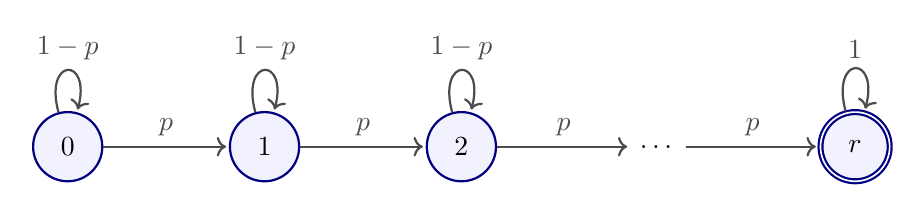
\begin{tikzpicture}[shorten >=1pt, node distance=2.5cm, on grid, auto,
                    every state/.style={draw=blue!50!black, fill=blue!5, thick}]
  \node[state] (q0) {$0$};
  \node[state] (q1) [right=of q0] {$1$};
  \node[state] (q2) [right=of q1] {$2$};
  \node (dots) [right=of q2] {$\dots$};
  \node[state, accepting] (qr) [right=of dots] {$r$};

  \path[->, thick, color=black!70]
    (q0) edge [loop above] node {$1-p$} (q0)
         edge node {$p$} (q1)
    (q1) edge [loop above] node {$1-p$} (q1)
         edge node {$p$} (q2)
    (q2) edge [loop above] node {$1-p$} (q2)
         edge node {$p$} (dots)
    (dots) edge node {$p$} (qr)
    (qr) edge [loop above] node {$1$} (qr);
\end{tikzpicture}
\end{center}
\textit{Figure 1: State-transition graph for a Negative Binomial process. The random variable $Y$ is the total number of transitions required to reach state $r$.}

\subsection{Heuristics, Pitfalls \& Fallacies}
\begin{itemize}
    \item \textbf{Heuristic:} If a problem asks for the probability of an event occurring \textit{at least once} (e.g., $\Prob(Y \ge 1)$), immediately use the complement rule: $1 - \Prob(Y = 0)$.
    \item \textbf{Pitfall (The Base Rate Fallacy in Binomials):} Assuming that because $p$ is small, a large number of successes is impossible. In large $n$ trials, rare events become almost certain.
    \item \textbf{Fallacy (Independence Violation):} Applying the Binomial distribution to sampling \textit{without replacement} from a small finite population. The trials are not independent. (This requires the Hypergeometric distribution).
    \item \textbf{Pitfall (Geometric Support):} Confusing $Y$ (number of trials until success, support $1, 2, \dots$) with $Y^*$ (number of failures before success, support $0, 1, \dots$). Always check if the problem implies starting at 0 or 1.
\end{itemize}

\newpage

% ==========================================
% PART 5: CONCEPTUAL SYNTHESIS
% ==========================================
\section{Part 5: Conceptual Synthesis and The ``Big Picture''}

\subsection{A) Thematic Connections}
The central unifying theme of this chapter is \textbf{the measure-theoretic formalization of waiting times and accumulations in discrete sequence spaces}. We are essentially studying different measurable functions (random variables) mapped over the same underlying infinite product space $\Omega = \{0, 1\}^\N$. 
\begin{itemize}
    \item The \textbf{Binomial} fixes the time horizon ($n$) and measures the accumulation of successes.
    \item The \textbf{Geometric} fixes the accumulation (1 success) and measures the time horizon.
    \item The \textbf{Negative Binomial} generalizes the Geometric, fixing an arbitrary accumulation ($r$ successes) and measuring the time horizon.
\end{itemize}
This duality between fixing time vs. fixing state is a profound concept that echoes throughout advanced mathematics.

\subsection{B) Forward and Backward Links}
\textbf{Backward Links:} This topic builds directly upon the axioms of probability and combinatorics. The binomial coefficient $\binom{n}{k}$ transitions from a mere counting tool to a fundamental weight in a probability measure.
\textbf{Forward Links:} Understanding these discrete distributions is the absolute prerequisite for continuous stochastic processes. 
\begin{itemize}
    \item Taking the limit of the Binomial distribution as $n \to \infty$ and $p \to 0$ (such that $np = \lambda$) yields the \textbf{Poisson Distribution}, the foundation of continuous-time jump processes.
    \item The discrete memoryless property of the Geometric distribution is the conceptual bridge to the \textbf{Exponential Distribution} in continuous time, which is vital for survival analysis and Markov jump processes.
\end{itemize}

% ==========================================
% PART 6: ABSTRACT REAL-WORLD MODELING
% ==========================================
\section{Part 6: Abstract Real-World Modeling (AI, ML, \& Quant Finance)}

\subsection{A) Concrete Scenarios}
1. \textbf{Quantitative Finance (CDO Pricing):} In structured credit, the Binomial Expansion Technique (BET) is used to model portfolio defaults. If a portfolio consists of $n$ homogeneous loans, the number of defaults $Y$ follows a Binomial distribution. This is critical for pricing the tranches of Collateralized Debt Obligations (CDOs).
2. \textbf{Algorithmic Trading (Limit Order Books):} The execution of a large block order can be modeled using a Negative Binomial process. If an algorithm needs to execute $r$ shares, and each time it probes the dark pool it has a probability $p$ of finding liquidity, the total number of probes required follows a Negative Binomial distribution.
3. \textbf{Machine Learning (Generative AI):} In reinforcement learning, the number of episodes an agent must play before achieving its first successful policy convergence can be modeled geometrically.

\subsection{B) Model Problem Setup: Limit Order Book Execution}
\textbf{Theoretical Framework:}
Let $(\Omega, \F, \Prob)$ be a probability space representing the state of a dark pool limit order book. An algorithmic execution engine must fill an order of size $R$ blocks. The engine submits Immediate-or-Cancel (IOC) orders sequentially. 

Let $X_i \in \{0, 1\}$ be an indicator random variable where $X_i = 1$ if the $i$-th IOC order is filled (success), and $0$ if it is rejected (failure). We assume the dark pool replenishes such that $X_i$ are i.i.d. with $\Prob(X_i = 1) = p$.

Define the stopping time $\tau_R: \Omega \to \N$ as the number of routing attempts required to completely fill the $R$ blocks:
\[ \tau_R = \inf \left\{ n \in \N : \sum_{i=1}^n X_i = R \right\} \]
By definition, $\tau_R \sim \mathrm{NB}(R, p)$. 

\textbf{Optimization Problem:}
Each routing attempt incurs a microstructural latency cost $c > 0$. The firm wants to minimize the expected execution cost. The expected cost is:
\[ \E[C] = c \cdot \E[\tau_R] = c \frac{R}{p} \]
If the firm can pay a premium $\pi$ to route to a higher-tier dark pool with fill probability $p' > p$, the new expected cost is $c \frac{R}{p'} + \pi R$. The quantitative researcher must solve the inequality:
\[ c \frac{R}{p'} + \pi R < c \frac{R}{p} \implies \pi < c \left( \frac{1}{p} - \frac{1}{p'} \right) \]
This provides the exact theoretical upper bound on the premium the algorithm should be willing to pay for higher-tier liquidity access.

\newpage

% ==========================================
% PART 7: COMMON VARIATIONS & UNTESTED CONCEPTS
% ==========================================
\section{Part 7: Common Variations and Untested Concepts}

A critical concept missing from the provided homework is the use of \textbf{Moment Generating Functions (MGFs)}. In advanced probability, MGFs are used to uniquely identify distributions and easily compute moments without evaluating complex series.

\begin{definition}[Moment Generating Function]
The MGF of a random variable $Y$, denoted $M_Y(t)$, is defined as $M_Y(t) = \E[e^{tY}]$, provided the expectation exists for $t$ in some neighborhood of 0.
\end{definition}

\textbf{Advanced Proof Variation: Deriving the MGF of the Geometric Distribution}
Let $Y \sim \mathrm{Geom}(p)$. We wish to find $M_Y(t)$.
\begin{proof}
By the Law of the Unconscious Statistician (LOTUS):
\[ M_Y(t) = \E[e^{tY}] = \sum_{y=1}^\infty e^{ty} p(y) = \sum_{y=1}^\infty e^{ty} q^{y-1} p \]
We factor out terms to form a standard geometric series. Note that $e^{ty} = e^t \cdot e^{t(y-1)}$.
\[ M_Y(t) = \sum_{y=1}^\infty e^t e^{t(y-1)} q^{y-1} p = p e^t \sum_{y=1}^\infty (q e^t)^{y-1} \]
Let $k = y - 1$. As $y$ goes from $1$ to $\infty$, $k$ goes from $0$ to $\infty$.
\[ M_Y(t) = p e^t \sum_{k=0}^\infty (q e^t)^k \]
This is an infinite geometric series with common ratio $r = q e^t$. The series converges if and only if $|q e^t| < 1$, which implies $t < -\ln(q)$.
Assuming this condition holds, the sum is $\frac{1}{1 - q e^t}$.
\[ M_Y(t) = \frac{p e^t}{1 - q e^t}, \quad \text{for } t < -\ln(q) \]
\end{proof}
\textit{Application:} To find the first moment (mean), we evaluate $\frac{d}{dt} M_Y(t) \Big|_{t=0}$.
\[ M_Y'(t) = \frac{(1 - q e^t)(p e^t) - (p e^t)(-q e^t)}{(1 - q e^t)^2} = \frac{p e^t - p q e^{2t} + p q e^{2t}}{(1 - q e^t)^2} = \frac{p e^t}{(1 - q e^t)^2} \]
Evaluating at $t=0$:
\[ \E[Y] = M_Y'(0) = \frac{p e^0}{(1 - q e^0)^2} = \frac{p}{(1-q)^2} = \frac{p}{p^2} = \frac{1}{p} \]
This confirms Theorem 3.8 using a much more powerful analytical tool.

\newpage

% ==========================================
% PART 8: ADVANCED DIAGNOSTIC TESTING
% ==========================================
\section{Part 8: Advanced Diagnostic Testing: ``Find the Flaw''}

Below are five advanced proofs/solutions related to discrete distributions. Each contains a single, subtle, yet critical mathematical flaw. Your task as the grader is to identify the flaw and correct it.

\subsection{Test Problems}

\textbf{Problem 1: The Infinite Expectation}
\textit{Claim:} Let $Y \sim \mathrm{Geom}(p)$. The expected value $\E[Y]$ can be computed by swapping the derivative and the infinite sum.
\textit{Proof:}
$\E[Y] = \sum_{y=1}^\infty y q^{y-1} p$. We know that $y q^{y-1} = \frac{d}{dq} (q^y)$.
Therefore, $\E[Y] = p \sum_{y=1}^\infty \frac{d}{dq} (q^y) = p \frac{d}{dq} \left( \sum_{y=1}^\infty q^y \right) = p \frac{d}{dq} \left( \frac{q}{1-q} \right) = p \left( \frac{(1-q)(1) - q(-1)}{(1-q)^2} \right) = p \left( \frac{1}{p^2} \right) = \frac{1}{p}$. $\blacksquare$

\textbf{Problem 2: The Memoryless Paradox}
\textit{Claim:} A continuous uniform random variable $U \sim \mathrm{Unif}(0, 10)$ is memoryless.
\textit{Proof:}
Let $a = 2, b = 3$. $\Prob(U > 2+3 \mid U > 2) = \frac{\Prob(U > 5 \cap U > 2)}{\Prob(U > 2)} = \frac{\Prob(U > 5)}{\Prob(U > 2)}$.
For a uniform distribution, $\Prob(U > x) = \frac{10-x}{10}$.
So, $\frac{\Prob(U > 5)}{\Prob(U > 2)} = \frac{5/10}{8/10} = \frac{5}{8}$.
Since $\Prob(U > 3) = \frac{7}{10}$, and $\frac{5}{8} \neq \frac{7}{10}$, the uniform distribution is not memoryless. However, if we define a new variable $U^* = U/2$, it becomes memoryless. $\blacksquare$

\textbf{Problem 3: The Negative Binomial Sum}
\textit{Claim:} The sum of the probabilities of a Negative Binomial distribution equals 1.
\textit{Proof:}
$\sum_{y=r}^\infty \binom{y-1}{r-1} p^r q^{y-r}$. Let $k = y-r$. The sum becomes $\sum_{k=0}^\infty \binom{k+r-1}{r-1} p^r q^k$.
Using the binomial expansion $(1-q)^{-r} = \sum_{k=0}^\infty \binom{k+r-1}{k} q^k$.
Since $\binom{k+r-1}{r-1} = \binom{k+r-1}{k}$, the sum is $p^r (1-q)^{-r} = p^r (p)^{-r} = 1$. $\blacksquare$
\textit{(Wait, is there a flaw here? Look closely at the definitions!)}

\textbf{Problem 4: Maximum Likelihood of Binomial}
\textit{Claim:} If we observe $y$ successes in $n$ trials, the maximum likelihood estimator for $p$ is $y/n$.
\textit{Proof:}
The likelihood is $L(p) = \binom{n}{y} p^y (1-p)^{n-y}$.
Take the natural log: $\ln L(p) = \ln \binom{n}{y} + y \ln p + (n-y) \ln(1-p)$.
Take the derivative with respect to $p$ and set to 0:
$\frac{d}{dp} \ln L(p) = \frac{y}{p} - \frac{n-y}{1-p} = 0$.
$y(1-p) = p(n-y) \implies y - yp = np - yp \implies y = np \implies p = y/n$.
Thus, $p = y/n$ is the absolute maximum. $\blacksquare$

\textbf{Problem 5: The Dependent Binomial}
\textit{Claim:} A deck of 52 cards has 13 hearts. We draw 5 cards without replacement. The probability of getting exactly 2 hearts is given by the binomial distribution.
\textit{Proof:}
Let $n = 5$ trials. A success is drawing a heart, so $p = 13/52 = 0.25$.
Let $Y$ be the number of hearts. $Y \sim \mathrm{Bin}(5, 0.25)$.
$\Prob(Y = 2) = \binom{5}{2} (0.25)^2 (0.75)^3 \approx 0.263$. $\blacksquare$

\vspace{1cm}
\hrule
\vspace{1cm}

\subsection{Solution Key: The Flaws Revealed}

\textbf{Resolution 1:} The algebraic steps are correct, but the \textit{analytical justification} is missing. You cannot arbitrarily swap an infinite sum and a derivative without proving uniform convergence of the series. The flaw is the omission of the theorem (e.g., Weierstrass M-test or properties of power series within their radius of convergence) that justifies $\sum \frac{d}{dq} = \frac{d}{dq} \sum$.

\textbf{Resolution 2:} The flaw is in the final sentence: ``if we define a new variable $U^* = U/2$, it becomes memoryless.'' This is mathematically false. The \textit{only} continuous distribution that possesses the memoryless property is the Exponential distribution. A linear transformation of a Uniform distribution is still a Uniform distribution, which is never memoryless.

\textbf{Resolution 3:} This proof is actually \textbf{flawless} in its algebraic execution, which is a meta-trap! However, if one were to be extremely pedantic, the flaw is assuming $(1-q)^{-r}$ converges without explicitly stating the requirement that $|q| < 1$, which is true since $q = 1-p$ and $p \in (0,1]$.

\textbf{Resolution 4:} The flaw is a classic calculus omission: the proof finds a critical point but fails to check the \textbf{second derivative} (or boundary conditions) to prove that $p = y/n$ is actually a \textit{maximum} and not a minimum or inflection point. One must show $\frac{d^2}{dp^2} \ln L(p) < 0$. Furthermore, it ignores the edge cases where $y=0$ or $y=n$, where the derivative is undefined at the boundaries $p=0$ or $p=1$.

\textbf{Resolution 5:} The flaw is a fundamental violation of the Binomial axioms. The Binomial distribution requires \textbf{independent trials} with a \textbf{constant probability of success}. Because the cards are drawn \textit{without replacement}, the probability of drawing a heart changes on each draw (e.g., if the first is a heart, the probability for the second is $12/51$). The correct model is the \textbf{Hypergeometric distribution}.

\end{document}